
\section{IAAS SERVICE ONTOLOGY}
\label{chap:ontology}

What is an ontology? An ontology is a specification of a conceptualization. According to Gruber \cite{OntologyDefinition} an ontology defines a set of representational primitives with which to model a domain of knowledge. These  primitives are typically classes (or sets), attributes (or properties), and relationships (or relations among class members). The definitions of the representational primitives include information about their meaning and constraints on their logically consistent application.

% http://tomgruber.org/writing/ontology-definition-2007.htm
% http://www.opengroup.org/soa/source-book/ontologyv2/intro.htm#fig_soa_ontology

% ontologie jine fieldy - medicina

In general, any enterprise application can benefit from use of ontologies. They are used in field of semantics-based health information systems, interoperable reference ontologies in biology and biomedicine as summarised in Open Biological and Biomedical Ontologies\cite{OBO}.

The formal definition of cloud computing ontology was introduced by Youseff \cite{OntologyComputing}. It maps the complete domain of Cloud computing from software to hardware resources. It is divided into 5 layers of services.

\begin{enumerate}
 \item Servers (physical and virtual)
 \item Core Infrastructure Services (DNS, NTP, config management) 
 \item Storage (NAS and SAN)
 \item Network (Routers, Switches, Firewalls, Load Balancers)
 \item Facilities (Power, Cooling, Space)
\end{enumerate}

The scope of IaaS Service Ontology covers the level 1 and 2 with core infrastructure services and servers running OpenStack services. The levels 3 and 4 with network and storage devices will be adopted in further versions of the ontology. The level 5 will be implemented as last as no services are directly configured.

\subsection{ONTOLOGICAL STANDARDS}

The ontologies define the relations between terms, but does not prescribe exactly how they should be applied. Following ontologies serve as the starting point for creating new ontologies including the IaaS Service Ontology.

%\subsubsection{Service-Oriented Architecture}
\textbf{Service-Oriented Architecture}
The SOA ontology specification was developed in order to aid understanding, and potentially be a basis for model-driven implementation of software systems. It is being developed by Open Group and was updated to version 2 in april 2014. The ontology is represented in the Web Ontology Language (OWL) defined by the World-Wide Web Consortium (W3C). The ontology contains classes and properties corresponding to the core concepts of SOA \cite{SOAOntology}.

%\begin{figure}[!h]
%\centering
%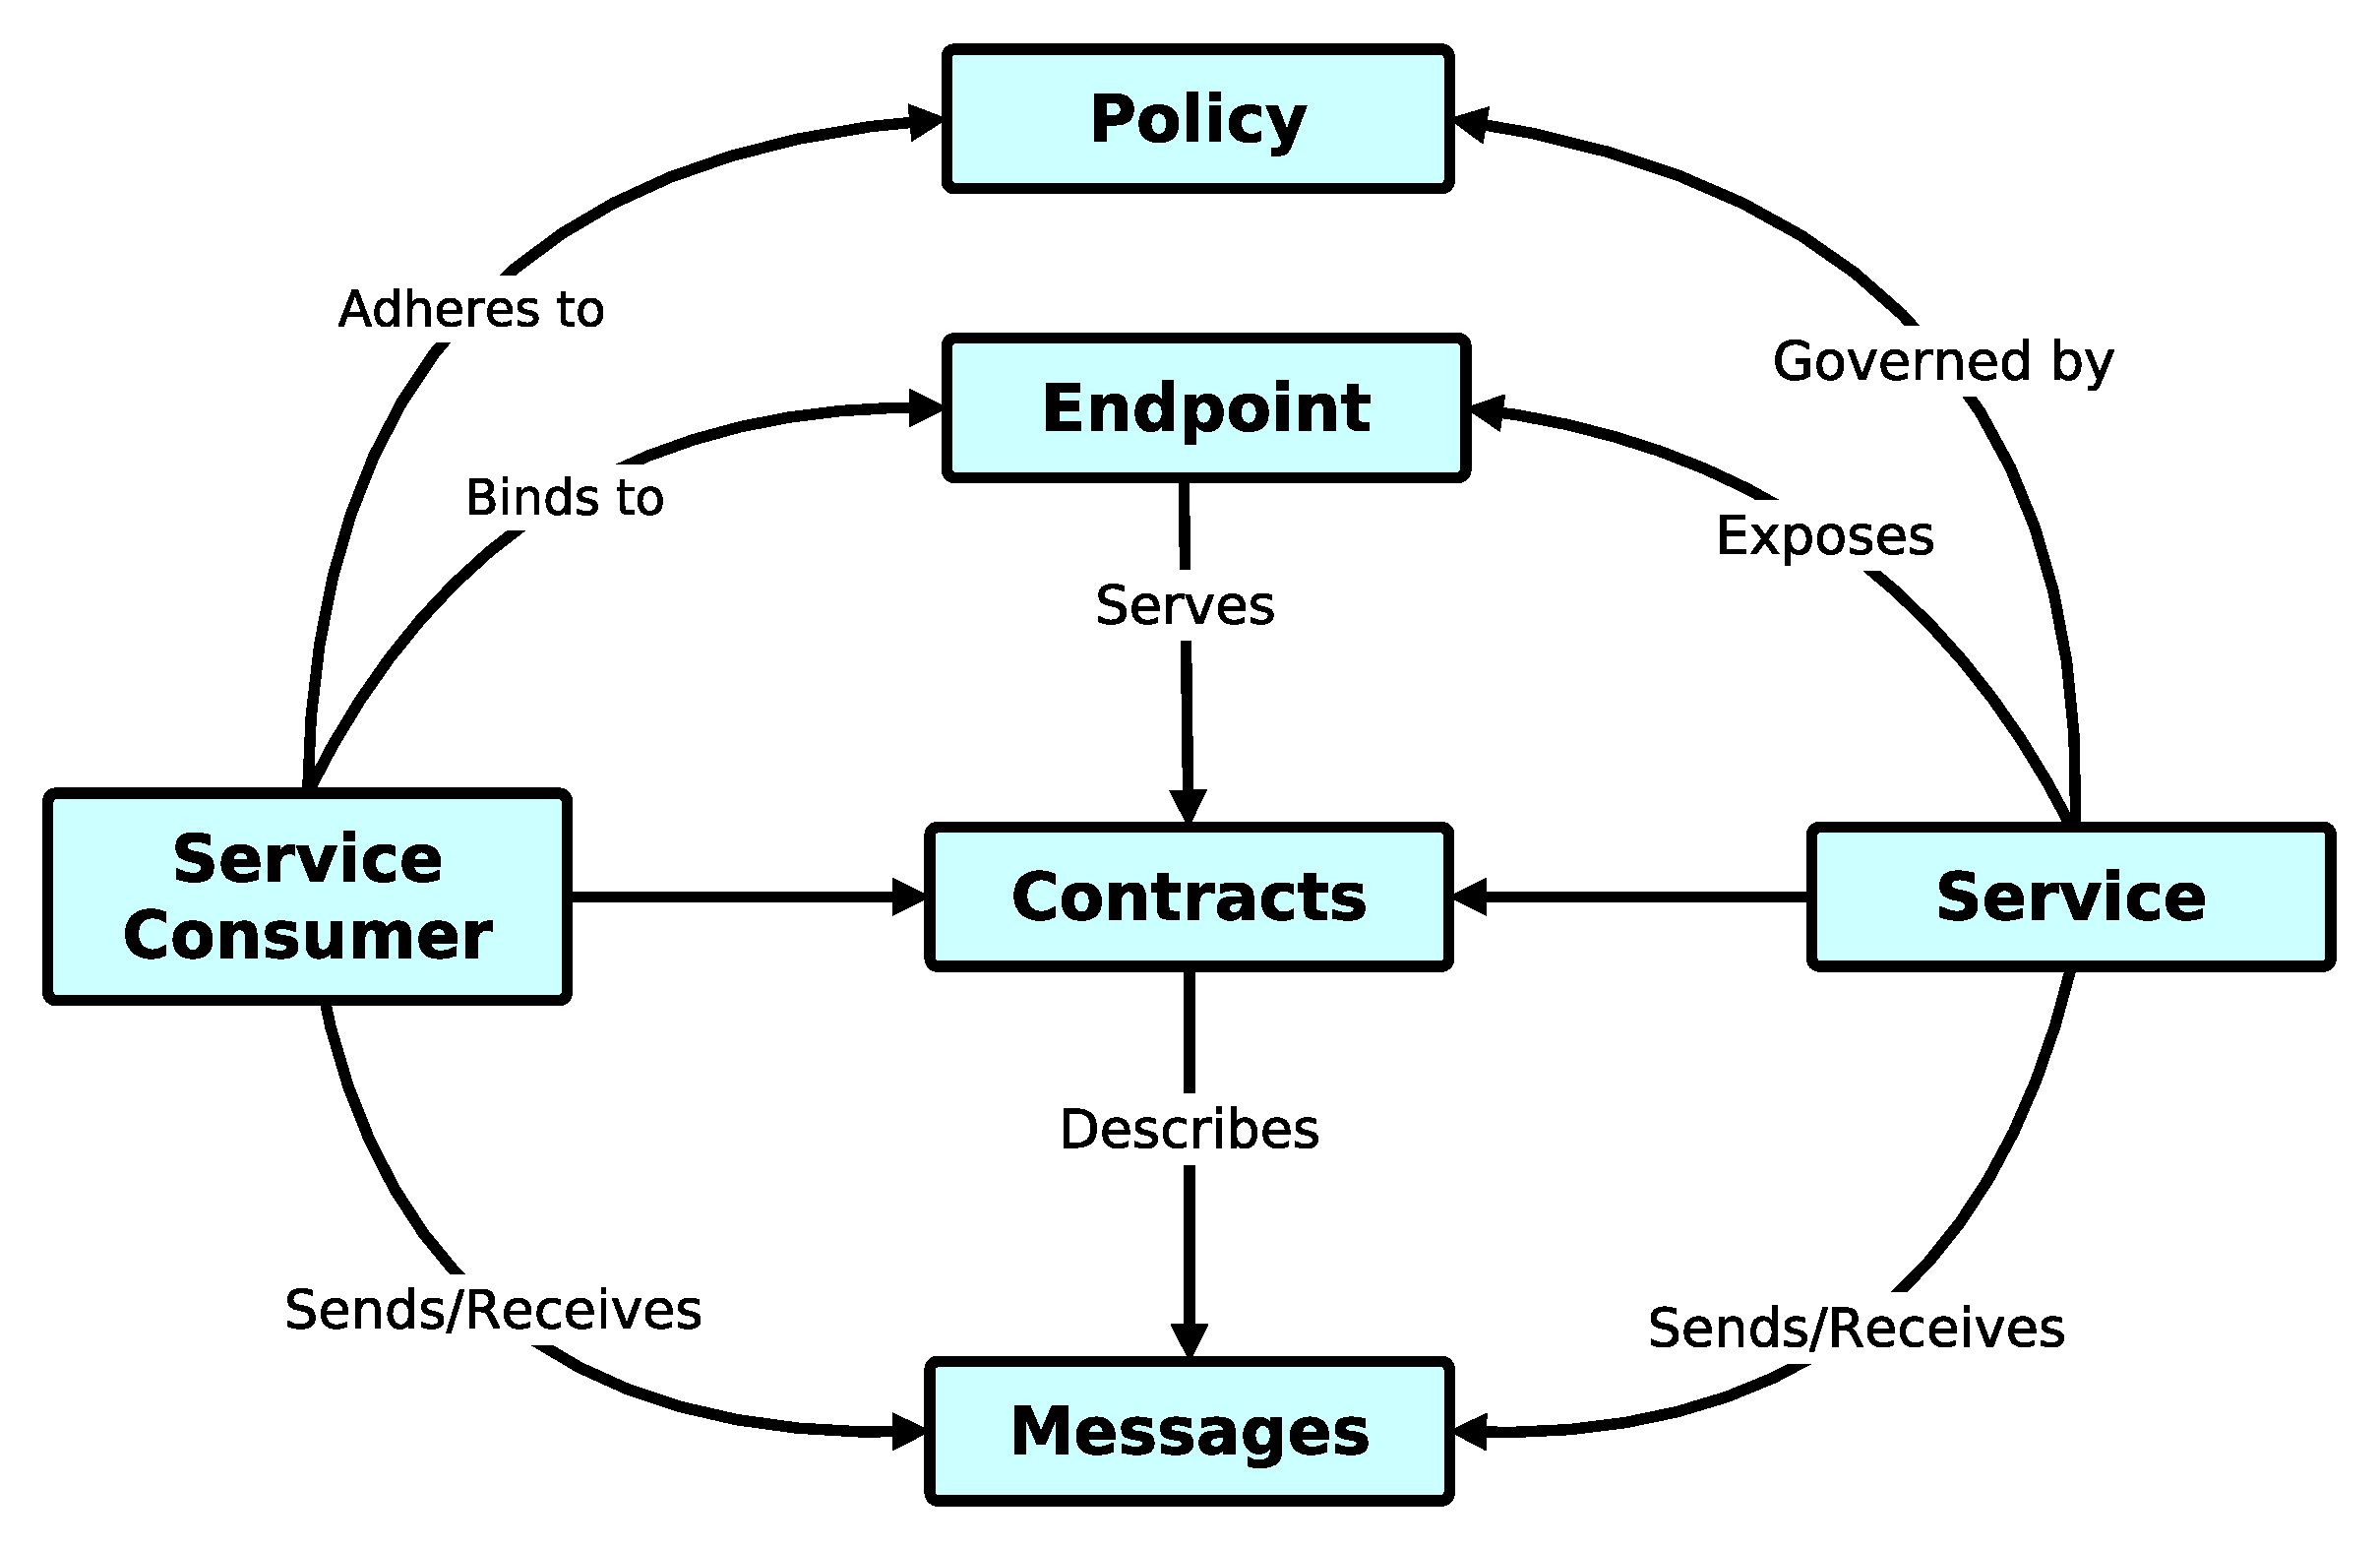
\includegraphics[scale=.2]{img/soa_relation.eps}
%\caption{SOA Sbject Property Service Interface}
%\label{fig:cm}
%\end{figure}

%\subsubsection{OSLC Configuration Management}
\textbf{OSLC Configuration Management}
OSLC Configuration Management Resource Definitions \cite{OasisCM} is a common vocabulary for versions and configurations of linked data resources. It provides suitable classes and properties from configuration management domain.

%\subsubsection{Dublin Core Metadata Initiative}
\textbf{Dublin Core Metadata Initiative}
The Dublin Core Metadata Intiative terms provide vocabularies for common resource definition. It is foundational meta-data vocabulary for many other schemas and covers the basic properties.

%\subsubsection{Basic Formal Ontology}

%The Basic Formal Ontology (BFO) is a formal ontological framework developed by Barry Smith and his associates that consists in a series of sub-ontologies at different levels of granularity. The ontologies are divided into two varieties:
% Continuant (or snapshot) ontologies, comprehending continuant entities such as three-dimensional enduring objects, and occurrent ontologies, comprehending processes conceived as extended through (or as spanning) time.

\subsection{ONTOLOGY SERIALIZATION FORMATS}

There are several ways how to serialize ontology. In it's core ontology representation is a linking structure that forms a directed, labeled graph, where the edges represent the named relation between two resources, represented by the graph nodes. This graph view is the easiest possible mental model for ontologies and is often used in easy-to-understand visual explanations. They differ by reading and writing speed. 

%- speed - parsing / scaling,  integration, maintenance costs, security issues

%\subsubsection{RDF/OWL-DL Documents}
\textbf{RDF/OWL-DL Documents}
Ontologies are stored in Web Ontology Language (OWL) defined by the World-Wide Web Consortium (W3C). OWL has three increasingly expressive sub-languages: OWL-Lite, OWL-DL, and OWL-Full \cite{OWL}. The sub-language OWL-DL provides the greatest expressiveness possible while retaining computational completeness and decidability. RDF is a standard model for data interchange, it as features that facilitate data merging even if the underlying schemas differ, and it specifically supports the evolution of schemas over time without requiring all the data consumers to be changed. The format is used by ontology editors

%\subsubsection{Graph Databases}
\textbf{Graph Databases}
Graph databases can store ontologies very well as they have graph format very similar to RDF format which is standard format of any XML based graph database, just very different implementation. Graph database uses graph structures with nodes, edges, and properties to represent and store data. A graph database is any storage system that provides index-free adjacency. This means that every element contains a direct pointer to its adjacent elements and no index lookups are necessary.

% http://en.wikipedia.org/wiki/Graph_database

% je to servica, tzn overhead oproti xml filu, ale zas ma api atd ...

\subsection{PLAIN META-DATA SERIALIZATION}

The domain of cloud computing services can be mapped not just by ontologies but in a less formal data structures. The most common examples are YAML or JSON files with plain or nested data structures. The schema is enforced by documentation and no semantic validation can be used.

%\subsubsection{Hierarchical Databases}
\textbf{Hierarchical Databases}
The more complex meta-data can be stored in hierarchical databases. These systems  allow to define service parameters through class inheritance, which can be overridden. Hierarchical classes can be featured as sets, commonalities, or as roles. You can assemble your infrastructure definition from smaller bits, eliminating duplication and exposing all important parameters to a single location. Within hierarchical databases parameters can reference other parameters in the very hierarchy that are actually assembling.

% http://reclass.pantsfullofunix.net/

%\subsection{Ontology structure}

%\begin{figure}[!h]
%\centering
%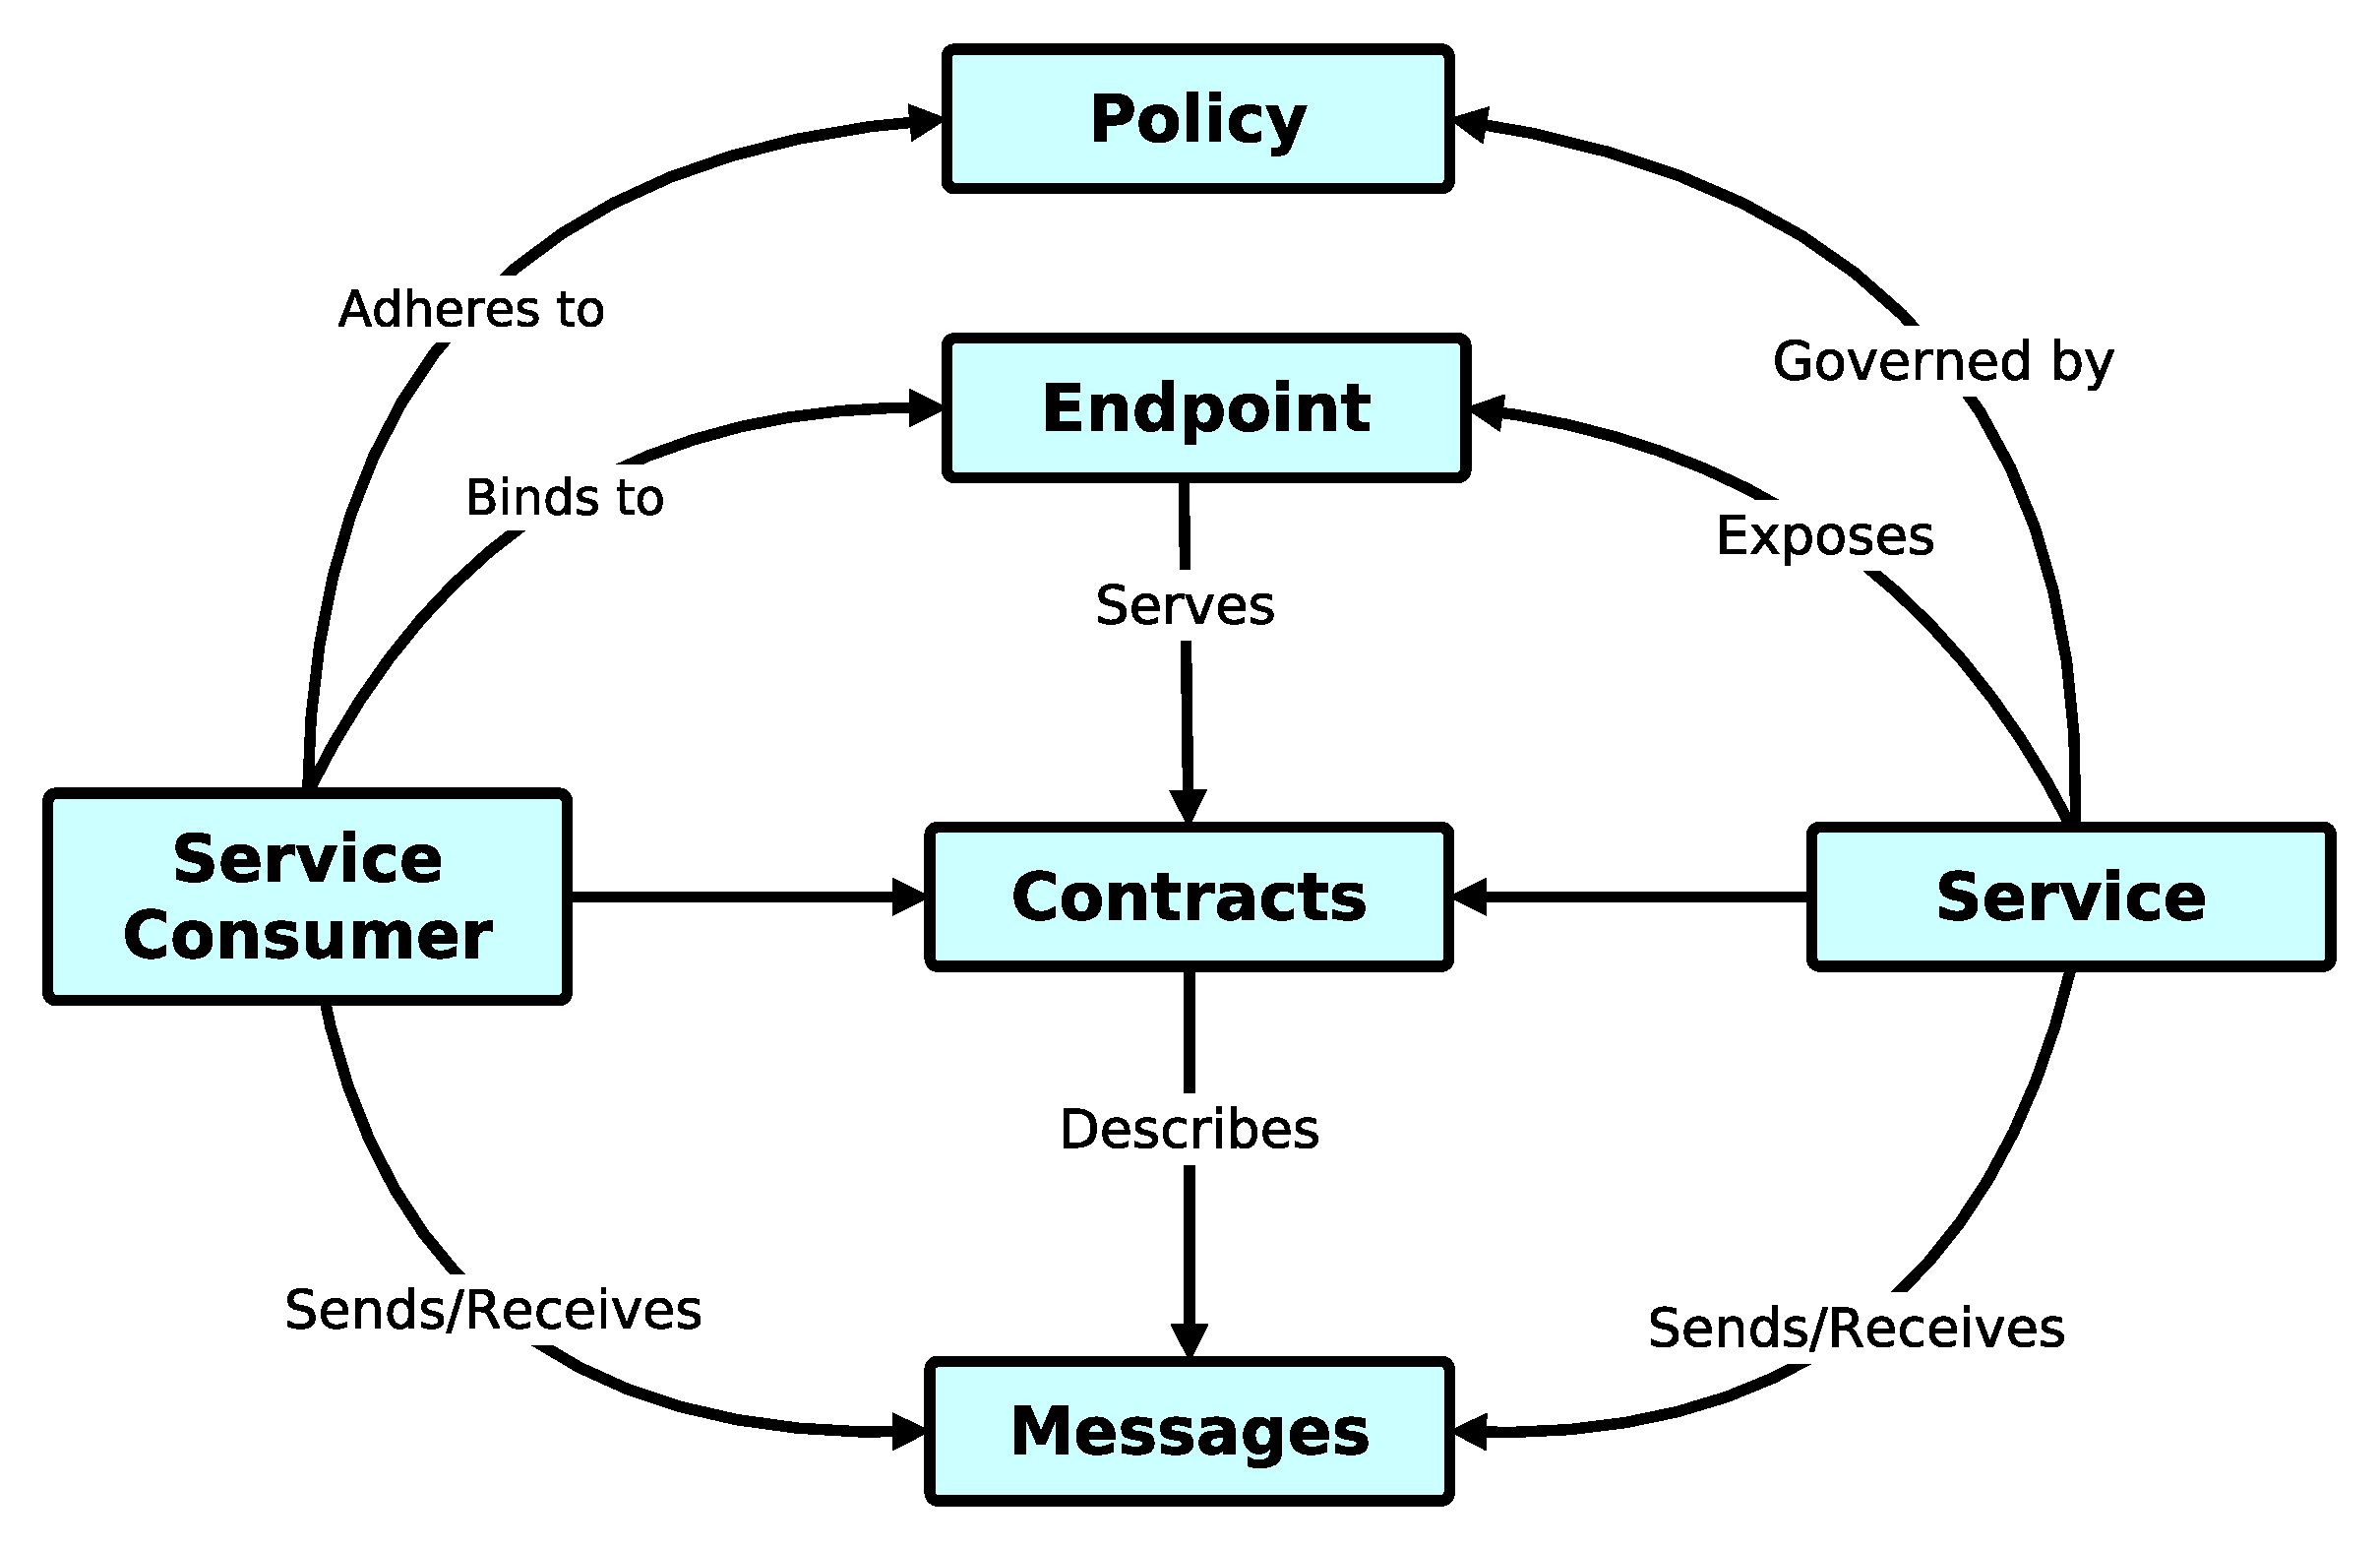
\includegraphics[scale=.2]{img/soa_relation.eps}
%\caption{SOA Sbject Property Service Interface}
%\label{fig:cm}
%\end{figure}

%\begin{figure}[!h]
%\centering
%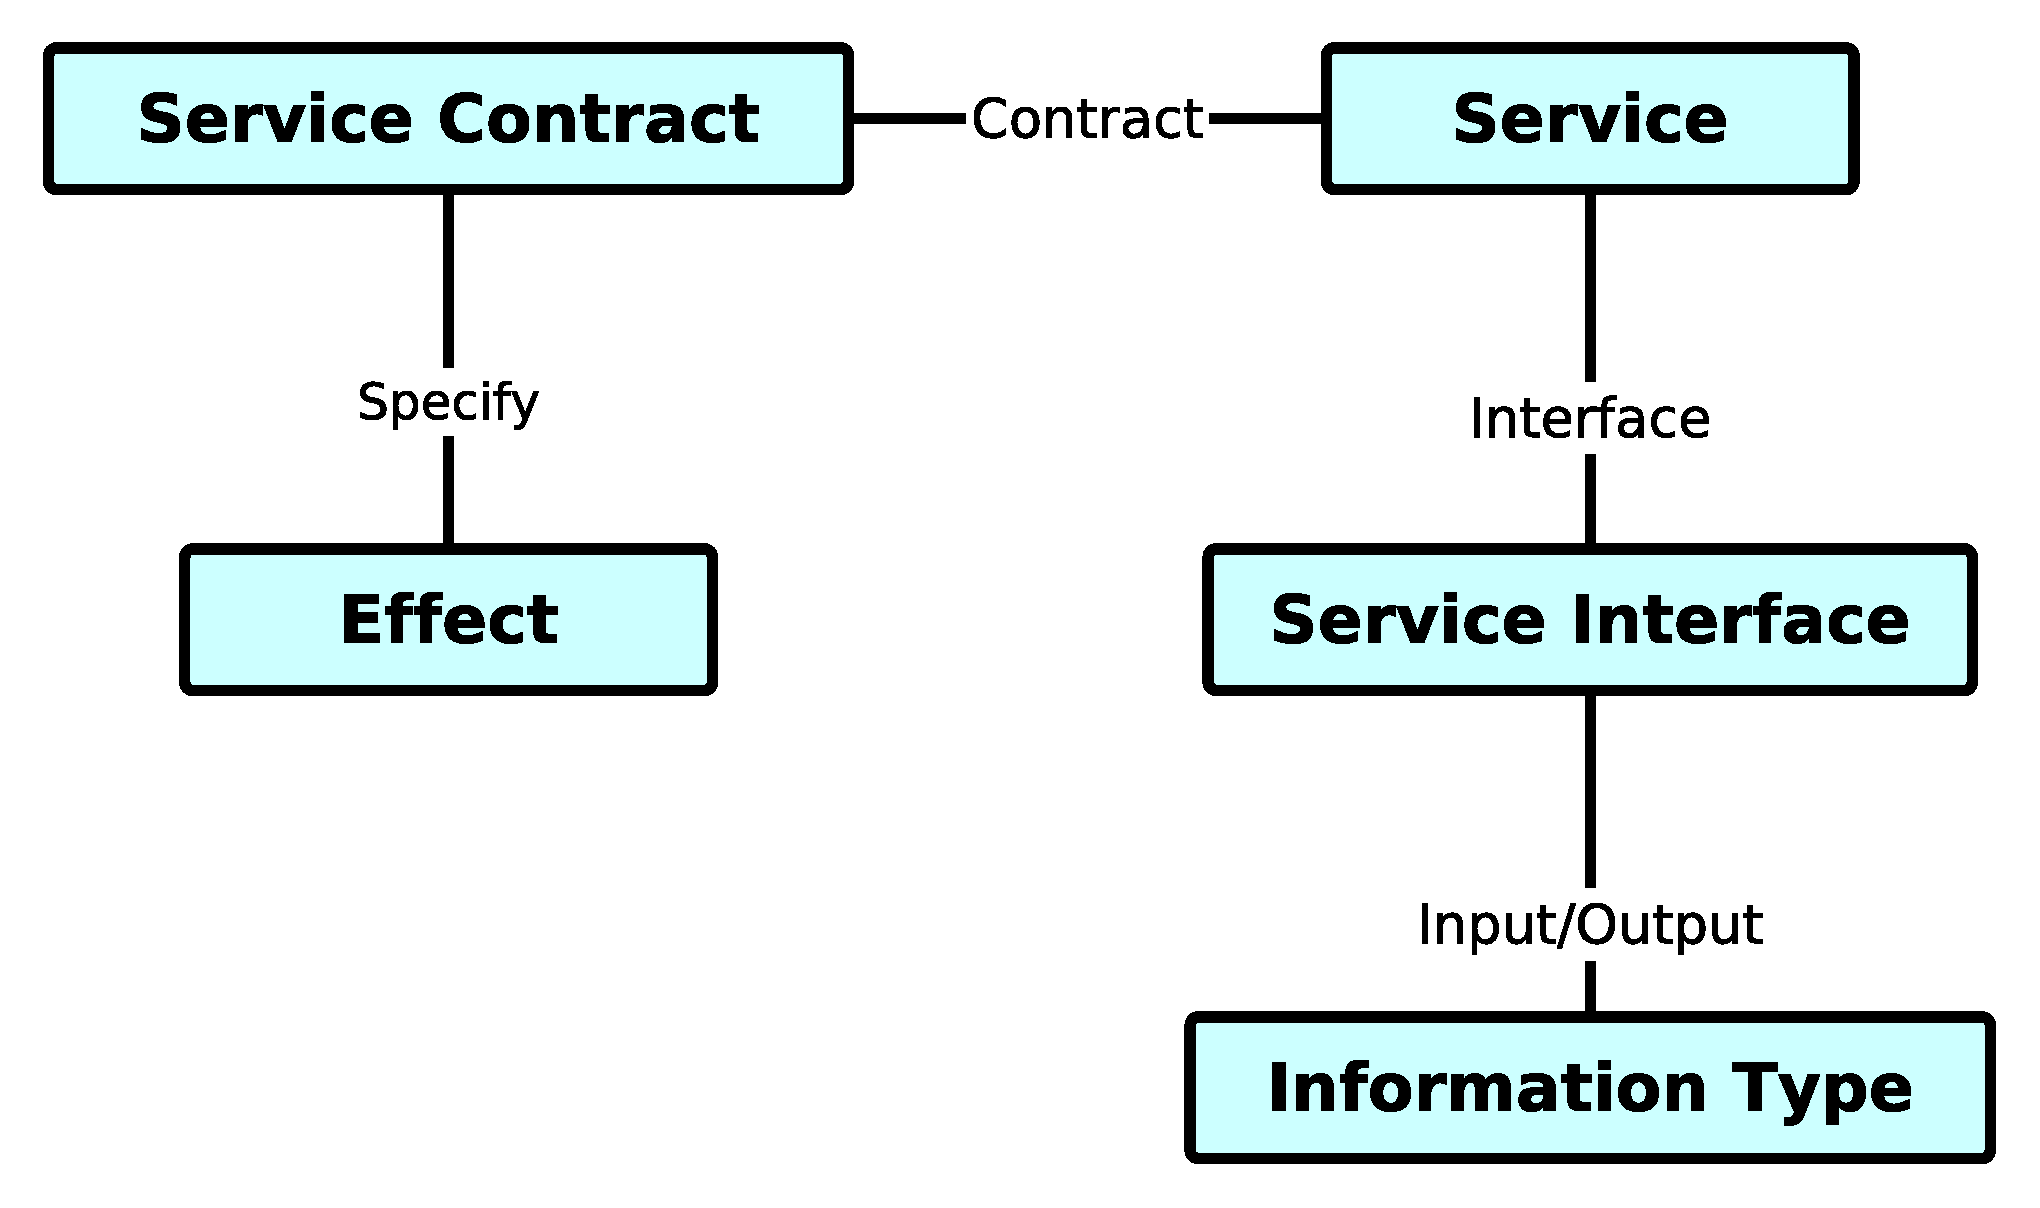
\includegraphics[scale=.2]{img/soa_property.eps}
%\caption{SOA service property}
%\label{fig:cm}
%\end{figure}

%\subsection{Comparison}

% Srovnání jednolivých formátů pro ontologii pro openstack řešení - bezpečnost, rychlost, integrace
